\chapter{Antecedentes}
En este capitulo se presenta a manera de resumen el trabajo realizado durante 
la etapa del desarrollo correspondiente a Trabajo Terminal 1. Primeramente se 
presenta la propuesta del trabajo, es decir la definición del problemas, la 
definición de algunos conceptos como son el videojuego, la cultura, las 
metodologías de desarrollo, la definición de la solución; después se procede en 
presentar los ajustes que se realizan en el proyecto una vez que se concluyo el 
periodo del trabajo terminal 1, tales como la asignación de trabajo, el enfoque 
del problema y la actualización del motor de juego; seguido de esto se presentan 
las observaciones realizadas por los sinodales durante la presentación del trabajo 
terminal 1 y como fueron solucionadas. Finalmente se hace un resumen del trabajo 
realizado durante el trabajo terminal 1, correspondiente a la etapa de 
preproducción y a los dos primeros sprints de la etapa de producción.   

\section{Propuesta}
En esta sección se presenta a manera de resumen las propuestas y los conceptos 
definidos durante el trabajo terminal 1, tales como el planteamiento del problema, 
conceptos y definiciones referentes al videojuego y su desarrollo, la definición 
y delimitación de la cultura y el planteamiento de la solución que se desarrolla 
durante el trabajo terminal.  

%====== Planteamiento del problema ======%
\subsection{Planteamiento del problema}
En México existe un fuerte desinteres y desconocimiento hacia su cultura e historia 
nacional. De acuerdo con la Tercera Encuesta Nacional de Cultura Constitucional, 
el 52.7 \% de los encuestados desconoce el año en que se aprobó la constituación 
nacional y no la relaciona con la Revolución Mexicana \cite{RefConsti}. Con base 
en la encuesta realizada por Parametría, empresa dedicada a la investigación 
estratégica de la opinión y análisis de resultados, solo el 32\% de su encuestados 
supó que México se independizó de España, el 51\% desconoce el país del que se 
independizó México, mientras que el resto del porcentaje de los encuestados 
piensa que México se independizó de otro país que no es España; la misma 
encuesta realizada por Parametría señala que el 25\% de los encuestados mencionaron 
personajes historicos ajenos a la independencia de México como participes de 
ésta y el 12\% respondió no saber que personajes historicos participaron en la 
independencia\cite{RefParametria}. 
 
%======Marco Teorico ======%
\subsection{Marco Teorico}
En esta sección se presentan los conceptos básicos para comprender el trabajo 
realizado durante el desarrollo del trabajo terminal, tales como la definición 
del videojuego, sus características, su clasificación, las metodologías de 
desarrollo, las herramientas para el desarrollo y la cultura. 

\subsubsection{Videojuego}
El grupo de periodista especializado en tecnología y desarrollo de software 
Carricay define al videojuego como: "una aplicación interactiva orientada 
al entretenimiento que, a través de ciertos mandos o controles, permite simular 
experiencias en la pantalla de un televisor, una computadora u otro dispositivo 
electrónico"\cite{Ref_DefVideo}.
\\
\par
Al igual que con otros productos tecnológicos, la evolución de los videojuegos 
ha sido vertiginosa, resultando complicado mencionar características comunes 
para todos los videojuegos. Sin embargo,en el libro “\textit{Marketing} y videojuegos: 
\textit{Product pacement, in-game, adevertising y 
advergaming}” se menciona que existen seis características comunes en los 
videojuegos: Interactividad, entretenimiento, jugabilidad, simulación \textbackslash 
virtualidad, inmersión y multiplataformidad\cite{RefCarac}; a continuación se 
menciona en que consisten cinco de las seis características, esto debido a que 
la última no se encuentra presente en todos los juegos y el mismo autor de la 
obra la menciona como una caracteristica opcional a tomar en cuenta:

	\begin{itemize}
		\item \textbf{Interactividad:} En el articulo "\textit{Defining Virtual Reality:
		 Dimensions Determining Telepresence}" se define la interactividad como la 
		 capacidad de los usuarios para participar y modificar la forma y el contenido 
		 de un entorno mediado en tiempo real\cite{RefInteractividad}.  
		
		\item \textbf{Entretenimiento:} en el articulo "Las Tecnologías del
		 Entretenimiento: Pasado, Presente y Futuro", el entretenimiento "se asocia, 
		 usualmente, de hacer algo que nos divierte, algo que podemos hacer solos o con 
		 otros, para entretenernos o divertirnos, en nuestro tiempo libre, o tal vez, 
		 algo que nos relaje o que nos haga reír"\cite{RefEntretenimiento}. 
		
		\item \textbf{Jugabilidad:} en el libro “\textit{Marketing} y videojuegos: 
	\textit{Product pacement, in-game, adevertising y advergaming}” se define la 
	jugabilidad como "la relación que existe entre todas las acciones reacciones e 
	interacciones tanto del videojugador como el videojuego como entre los propios 
	sistemas y subsistemas programados en el videojuego"\cite{RefCarac}.		
	
		\item \textbf{Simulación \textbackslash Virtualidad:} La simulación "se trata 
		de una representación a medida cuyo objetivo nos permite interactuar y 
		relacionarnos con lo representado según nuestros intereses"\cite{RefCarac}.
		
		\item \textbf{Inmersión:} Con base en el libro "La vida en la pantalla: La
		 construcción de la identidad en la era de internet", la inmersión es un 
		 proceso psicológico que se produce cuando la persona deja de percibir de 
		 forma clara su medio natural al concentrar toda su atención en un objeto,
		  narración, imagen o idea que le sumerge en un medio artificial 
		  \cite{RefInmersion}. Por su parte en la tesis "Libertad dirigida: Análisis 
		  formal del videojuego como sistema, su estructura y su avataridad", la 
		  inmersión se entiende como la coherencia de la ficción del juego y su 
		  aceptación por el jugador.\cite{refInmersionNavarro}  
	\end{itemize} 

Los videojuegos pueden se clasificados con base a su jugabilidad, en el libro 
"Juego. Historia, Teoría y Práctica del Diseño Conceptual de 
Videojuegos"\cite{Ref_JuegoDisenio} se propone la siguiente clasificación.
	\begin{itemize}
		\item \textbf{Juegos de acción:} Son juegos usualmente de temática 
				violenta. El jugador lucha por su supervivencia, para ello se vale 
				de armas o habilidades de  combate. 
			%==== Juegos de estrategia ====%
				\item \textbf{Juegos de estrategia:} Para que el jugador logre sus 
				objetivos en este tipo de juegos, éste debe de planear una estrategia, 
				normalmente a lago plazo. 
			%==== Juegos de Rol ====%
				\item \textbf{Juegos de Rol:} La mecánica de los juegos de rol gira 
				en torno a un grupo de héroes, con habilidades y progresión definidos; 
				el grupo de héroes debe de trabajar coordinadamente para cumplir un 
				objetivo; estos héroes pueden ser controlados por un solo jugador o 
				por varios. El jugador deberá explorar un mundo de gran tamaño 
				haciendo evolucionar a	sus personajes y sus habilidades. 
				\item \textbf{Videojuego de aventura:} Son parecidos a los juegos de 
				Rol; con la peculiaridad de que tienen una progresión más lineal y no 
				se hace tanto énfasis en los combates, siendo su eje principal la 
				narrativa.
				\item \textbf{Videojuegos de deportes:} Son todos aquellos videojuegos 
				que tratan sobre deportes que no involucren la conducción de un 
				vehículo. Pueden ser juegos sobre fútbol, fútbol americano, tenis, etc.
				\item \textbf{Videojuegos de carreras de vehículos:} Son todos aquellos 
				se centran en las carreras con todo tipo de vehículos, mayoritariamente 
				automóviles.
				\item \textbf{Videojuegos {\it puzzle:}} Este tipo de juego involucra 
				la resolución de un problema a partir de la utilización de una serie 
				limitada de recursos, por lo que si los recursos no se utilizan de la 
				manera correcta el problema no podrá ser solucionado.  
	\end{itemize}
	
Dentro de la clasificación de los juegos de acción entren los juegos de plataforma, 
definidos por una jugabilidad donde el jugador debe de controlar a un personaje 
con el que se dezplazará saltando entre plataformas y esquivando todo tipo de 
obstáculos y enemigos\cite{Ref_JuegoDisenio}. 
Es importante que se entienda el concepto del videojuego, sus características, 
su clasificación y la jugabilidad básica de un juego de plataforma ya que el 
presente Trabajo Terminal gira entorno al desarrollo de un videojuego de plataforma.

\subsubsection{Metodología de desarrollo}
Las metodologías de desarrollo de software son un conjunto de procedimientos, 
técnicas y ayudas a la documentación para el desarrollo de productos software
\cite{Ref_metodologia}. Para el presente trabajo terminal se consideran las 
siguientes metodologías como candidatas a implementar para guiar el desarrollo:

\begin{itemize}
	\item \textbf{Metodología en cascada:} Sigue una progresión lineal por lo que 
	cualquier error que no se haya detectado con antelación afectara todas las 
	fases que le sigan provocando una redefinición en el proyecto y por ende un 
	aumento en los costos de producción del sistema \cite{Ref:CarCascada}.Esta 
	metodología se divide en las siguientes etapas:
		\begin{itemize}
			\item \textbf{Análisis de los requisitos del software.}
			\item \textbf{Diseño.}
			\item \textbf{Codificación.}
			\item \textbf{Pruebas.}
			\item \textbf{Mantenimiento.}
		\end{itemize}
	\item \textbf{Metodología en \textit{Scrum}:} \textit{Scrum} parte de la visión 
	general que se desea que el producto alcance; a partir de esta visión se inicia la 
	división del proyecto en diferentes módulos. \textit{Scrum} implementa una 
	jerarquía entre los módulos en donde los módulos de mayor jerarquía son los 
	que se desarrollaran al inicio del proyecto o durante las primeras iteraciones 
	o \textit{sprints} \cite{Ref_ScrumRef}.Cada sprint se compone de las siguientes 
	fases:
	\begin{itemize}
		\item \textbf{Concepto}.
		\item \textbf{Especulación}.
		\item \textbf{Exploración}.
		\item \textbf{Revisión}.
		\item \textbf{Cierre}\cite{Ref_ScrumGuia}. 
	\end{itemize}
	\item \textbf{Metodología de Programación extrema:} Es una metodología de 
	desarrollo ágil y adaptable, soporta cambios de requerimientos sobre la marcha. 
	Su principal objetivo es aumentar la productividad y minimizar los procesos 
	burocráticos, por lo que el software funcional tiene mayor importancia que la 
	documentación\cite{Ref_XP}.
	\item \textbf{Metodología \textit{Huddle}:} Es una metodología cuya funcionalidad 
 se basa en la metodología \textit{Scrum}, con la diferencia de que está orientada al
  desarrollo de videojuegos.  De naturaleza ágil, resulta óptimo para equipos 
  multidisciplinarios de 5 a 10 personas; es iterativa, incremental y evolutiva 
  \cite{Ref_Huddle}. \textit{Huddle} se divide en las siguientes etapas:
  	\begin{itemize}
  		\item \textbf{Preproducción}.
		\item \textbf{Producción}.
		\item \textbf{Postmorten}.
  	\end{itemize}
\end{itemize}

Tras un riguroso análisis comparativo entre metodologías, se elige a 
\textit{Huddle}  como la metodología a guiar el desarrollo del Trabajo Terminal; 
esta elección se basa principalmente en que dicha metodología esta enfocada a 
videojuegos y no requiere ser adaptada por lo que se puede llevar a cabo el 
proyecto de manera directa sin tener que invertir tiempo en adaptar la metodología 
a las necesidades del desarrollo de un videojuego.

\subsubsection{Herramientas de desarrollo}
Como cualquier desarrollo de software, el desarrollo de un videojuego requiere 
se software especializado tal como un motor de juego, editores de imágenes, software 
de diseño, de edición de audio, etc. En este apartado se van a definir algunas de 
las herramientas utilizadas durante la elaboración del trabajo terminal.
\\
\par
La primera herramienta a definir es el del motor de juego. El motor de juego, 
también conocido como \textit{Game Engine}, parte del concepto de reutilización; 
es decir, es posible generar juegos a partir de un código base y común mediante una 
separación adecuada de los componentes fundamentales, tal como visualización de 
gráficos, control de colisiones, físicas, entrada de datos etc \cite{Ref:MutorGraf}; 
esto permite a quienes trabajen en un juego puedan centrarse en todos aquellos 
detalles que hacen al juego único. Dentro del mercado existen diferentes 
opciones de motores de juego tales como \textit{Unity3D}, \textit{UnrealEngine} 
y \textit{CryEngine}, por citar algunos. Para el presente trabajo terminal se 
decide por utilizar \textit{Unity3D} ya que ofrece: 

	\begin{itemize}
		\item Desarrollo muliplataforma, lo que permite aumentar la escalabilidad 
		del proyecto. 
		\item Curva de aprendizaje rápido.
		\item Comunidad de desarrolladores activa.
		\item Tres opciones de lenguajes de programacion para utilizar: 
		\textit{$\sharp C$,javaScript y Boo}.
		\item No requiere de muchos recursos para su instalación.
		\item Uso de diferentes tipos de licencia lo que permite contar con una 
		licencia gratuita, de pago y una de negocios. No existiendo mucha diferencia 
		de funcionalidad entre la licencia libre y la de pago.
	\end{itemize}
 En lo que refiere a la creación del entorno gráfico del videojuego, es decir de 
 sus sprites, se decide utilizar los \textit{software} de diseño 
 \textit{Adobe Phtoshop} y \textit{Corel Draw}. Ya que al momento de elegir dichos 
 softwares ya se contaba con experiencia previa sobre su funcionamiento y no 
 requiere ningún tipo de periodo de prueba para familiarizarse con su funcionamiento. 
 Ambos \textit{softwares} son de pago y para el desarrollo del presente trabajo 
 terminal se utiliza una licencia personal por lo que si se desea comercializar 
 el juego va a ser necesario adquirir otro tipo de licencia para le generación 
 de \textit{sprites}.


\subsubsection{Cultura}
Una vez explicado lo que es el videojuego, su metodologia de desarrollo y las 
herramientas a usar para desarrollarlo, es preciso definir lo que es la cultura; 
para tal objetivo el presnete trabajo se vale de la definición propuesta por la 
Organización de las Naciones Unidas para la Educación, la Ciencia y la Cultura 
(UNESCO, por sus siglas en ingles). La UNESCO define la cultura como “el conjunto 
de los rasgos distintivos, espirituales y materiales, intelectuales y afectivos 
que caracterizan a una sociedad o un grupo social. La cultura engloba, además 
de las artes y las letras, los modos de vida, los derechos fundamentales al ser 
humano, los sistemas de valores, las tradiciones y las creencias; de igual forma 
la cultura da al hombre la capacidad de reflexionar sobre sí mismo\cite{RefCultura}”. 
Bajo su misma definición la UNESCO, se plantea que la importancia de la cultura 
radica en su capacidad de hacer a los seres humanos racionales, críticos y 
éticamente comprometidos; ya que, través de ella se disciernen los valores y se 
efectúan opciones. Siendo por medio de ella que el hombre se expresa, toma conciencia 
de sí mismo, se reconoce como un proyecto inacabado, pone en cuestión sus propias 
realizaciones, busca incansablemente nuevas significaciones, y crea obras que lo 
trascienden \cite{RefCultura}.
\\
\par
Para efectos del presente trabajo terminal, este únicamente va a abordar la cultura 
de carácter historica, es decir la cultura que hace referencia a la herencia social, 
es decir aquella que relaciona a la sociedad con su pasado
\cite{RefculturaClasificacionEl}.

\subsection{Planteamiento de la solución}
Con el fin de fomentar la cultura y la historia se desarrolla Yolotl, un videojuego 
de plataforma y aventuras en dos dimensiones para dispositivos móviles android 5.1 
de gama media alta.
\\
\par
Las razones por las que se aborda la solución del problema con un videojuego se 
debe principalmente a diferentes factores tales como:

\begin{itemize}
	\item \textbf{El estado de la industria mexicana de los videojuegos:} En el 
	2017 México ocupó el 12 puesto en cuanto a consumo de videjuegos percibiendo 
	un ingreso de 1.4 mil millones de dolares en esta industria. A su vez México 
	cuenta con 49.2 millones de jugadores\cite{Ref_JuegosGanancia}.

	\item \textbf{El auge de los juegos para teléfonos móviles:} En el 2017 la 
	industria del videojuego tuvo ganancias de 108.9 mil millones de dolares de 
	los cuales el 32\% de las ganancias fueron generadas por los teléfonos 
	inteligentes y un 10\% por las tablets; con este porcentaje los teléfonos 
	superaron a las consolas de mesa en ingresos\cite{Ref_JuegosGanancia}. 

	\item \textbf{El consumo de teléfonos móviles en México}: En el 2017 México 
	contaba con 52 millones de usuarios de teléfonos móviles, lo que lo ubicó en 
	el 9 puesto a nivel mundial en el consumo de teléfonos inteligentes
	\cite{Ref_TelefonosGanancia}.

	\item \textbf{La interactividad de un videojuego:} Como se menciona en el 
	artículo \textit{Identification with the Player Character as Determinant 
	of VideoGames Enjoyment}: en los videojuegos, la interactividad juega un 
	papel importante para identificar y adoptar un determinado concepto, ya que 
	dentro del videojuego el jugador no es un espectador, pues participa 
	directamente en la historia e interactúa con el mundo del personaje; esto 
	genera una relación íntima entre el jugador y el personaje puesto que es 
	gracias al jugador que el personaje puede avanzar en la historia y a su vez 
	es gracias al personaje que el jugador puede interactuar con la historia
	\cite{PlayerIdentification}. 
\end{itemize}
\section{Ajustes}
En esta sección se definen todas las nuevas estrategias a seguir para agilizar y 
optimizar el desarrollo del juego.

\subsection{Correción del enfoque de la solución}

\subsection{Nueva división de trabajo}
Antes del inicio del tercer \textit{sprint} y teniendo como base la experiencia 
de desarrollo los anteriores prototipos, queda claro que se necesita diseñar una 
nueva estrategia que permita agilizar el desarrollo del juego sin comprometer 
la calidad del mismo. Por tal motivo se decide reorganizar la asignación de 
tareas, en lugar de que los miembros del equipo de desarrollo se encarguen del 
mismo nivel, se reparten los niveles restantes del desarrollo entre los 
integrantes del equipo. Quedando la asignación de los niveles como se ve en la 
figura \ref{fig:Tareas} .

		\begin{figure}[h]
    			\centering
    			\includegraphics[width=0.8\textwidth]{02Antecedentes/Imagenes/tareasAsignacion.png}
    			\caption{Asignacion de tareas}
    			\label{fig:Tareas}
		\end{figure}


Esta división de trabajo permite que los niveles se desarrollen de manera paralela y no de manera secuencial como se había trabajado hasta este \textit{sprint}; simulando de esta forma un flujo de trabajo similar a procesamiento multihilo, en el que cada integrante del equipo es un hilo y desarrolla sus tareas de manera paralela al otro.

\subsection{Actualizando el motor de juego}
Paralelamente a la nueva asignación de tareas, fue liberada la versión 
2017.3.1f de \textit{Unity3D}. Esta versión incluye herramientas que agilizan la 
creación de niveles como el uso de: 
	\begin{itemize}
		\item \textbf{\textit{Tilemap}:} Herramienta para el mapeado de niveles. Esta 
		herramienta facilita la creación de mapas al crear una malla sobre la que 
		se arrastraran diferentes \textit{Sprites} que se hayan importado previamente 
		al tilemap (ver figura \ref{fig:TilemapPantalla}). En la sección () se 
		profundizará su funcionamiento.
		
		\begin{figure}[h]
    			\centering
    			\includegraphics[width=0.6\textwidth]{02Antecedentes/Imagenes/tilemaps01.png}
    			\caption{Vista de la escena cuando se tiene un \textit{GameObject} de 
    			tipo \textit{Tilemaps} para la construcción de niveles}
    			\label{fig:TilemapPantalla}
		\end{figure}
		
		\item \textbf{\textit{Cinemachine}:} \textit{Asset} que permite controlar la 
		cámara de la escena, con este \textit{asset} se le puede indicar que objeto se 
		desea que la cámara siga y se puede asignar un área que limitara el movimiento 
		de la cámara (ver figura \ref{fig:CinemaPantalla}). \textit{Cinemachine} se 
		descarga directamente desde la tienda de \textit{assets} de \textit{Unity} y 
		fue desarrollado por los ingenieros de \textit{Unity}, lo que significa que 
		no genera conflictos o no requiere de configuraciones extras al proyecto para 
		importar. En la sección () se profundizará su funcionamiento.
			
			\begin{figure}[h]
    			\centering
    			\includegraphics[width=0.6\textwidth]{02Antecedentes/Imagenes/cinemachine01.png}
    			\caption{Vista de la escena cuando se tiene un \textit{GameObject} de 
    			tipo \textit{Tilemaps} para la construcción de niveles}
    			\label{fig:CinemaPantalla}
			\end{figure}

		\item \textbf{\textit{Sprite Packer}}: Si bien no es una herramienta para 
		construcción de niveles o un \textit{asset}, esta herramienta es una de las 
		más útiles que se agregó a la nueva versión de \textit{Unity} ya que, como 
		su nombre lo indica, permite el empaquetado de \textit{sprites} (ver figura ). 
		Empaquetar 
		los \textit{sprites} es una práctica que optimiza el renderizado de objetos, 
		ya que el controlador de gráficos de \textit{Unity} realiza una sola llamada 
		por paquete cuando renderiza los objetos y con esa única llamada renderiza todos 
		los objetos de la escena que se encuentren en ese paquete; si los 
		\textit{sprites} no se encontraran dentro de un paquete el controlador de 
		gráficos de \textit{Unity} haría una llamada por cada \textit{sprite}.  
			\begin{figure}[h]
    			\centering
    			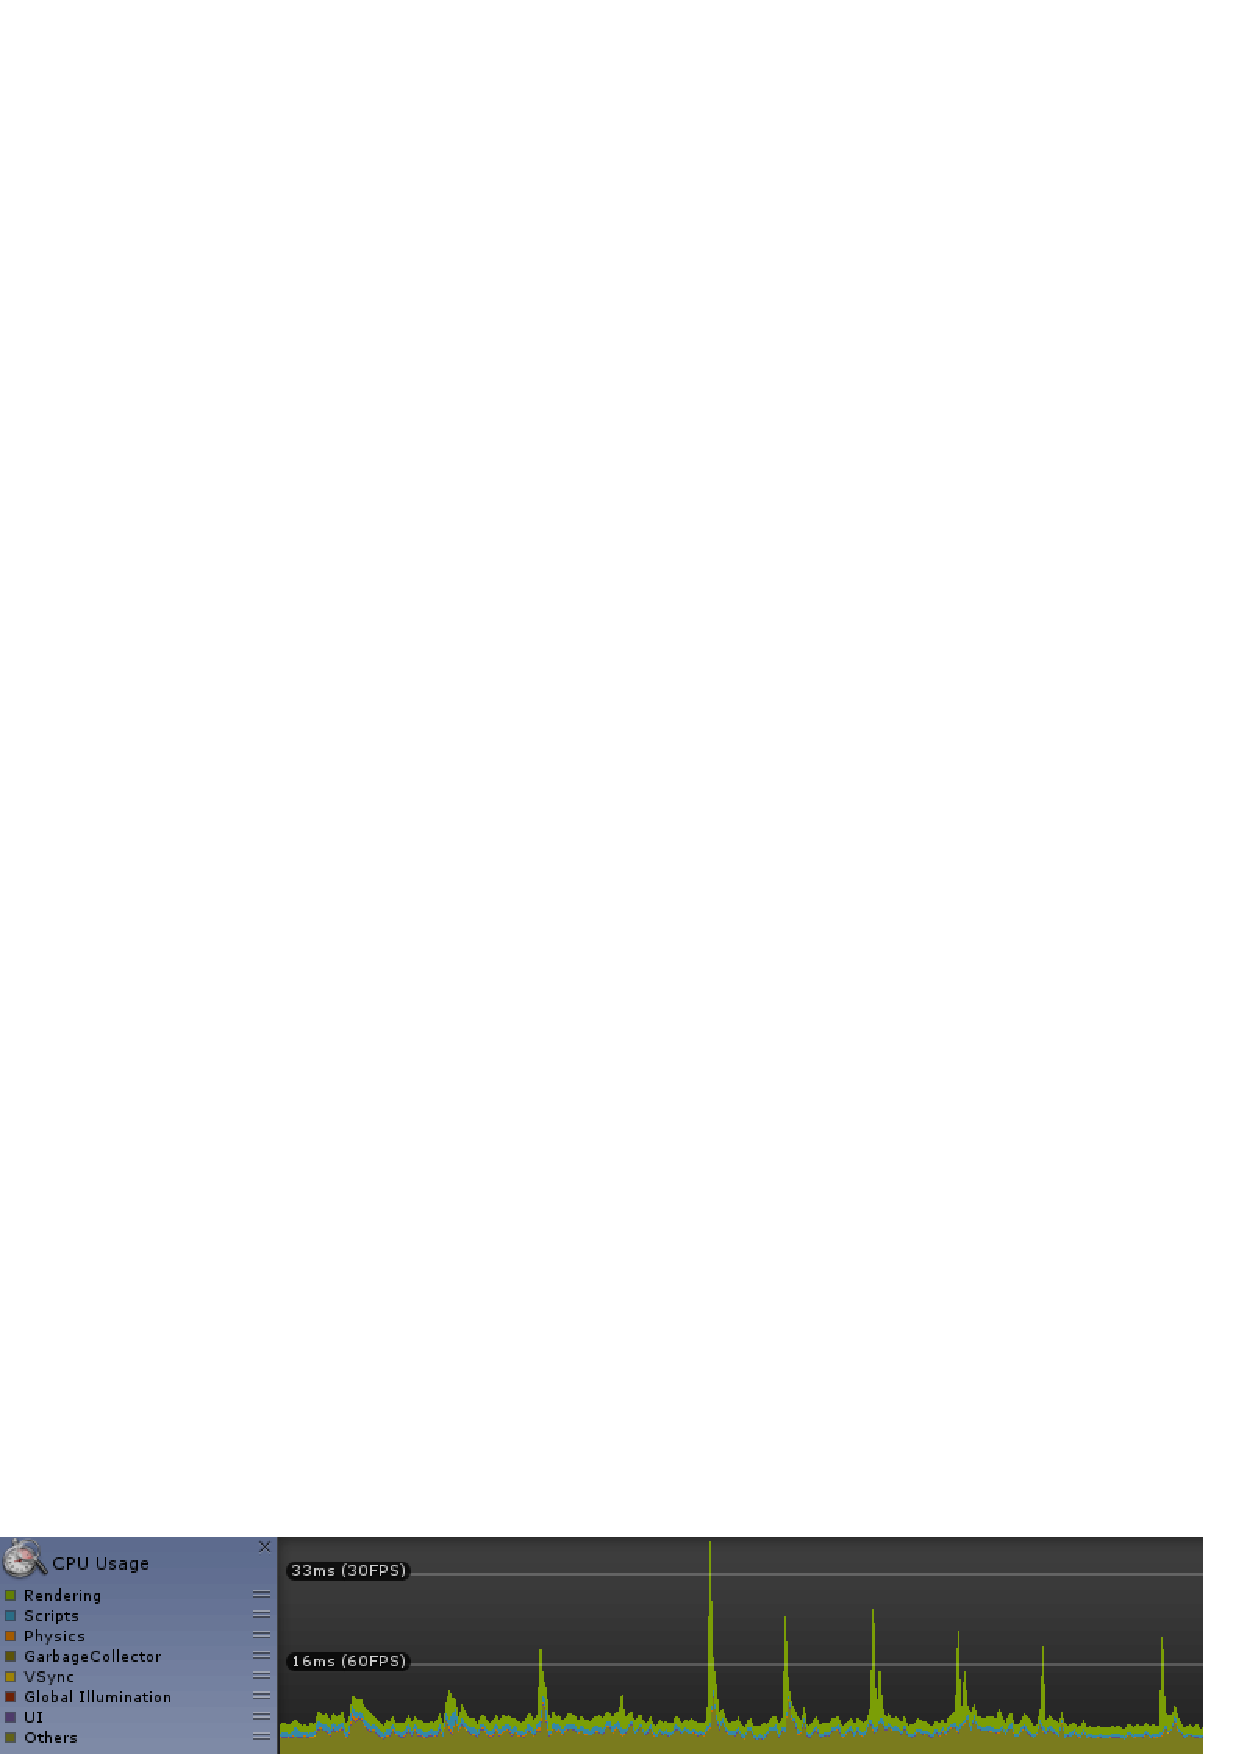
\includegraphics[width=0.6\textwidth]{02Antecedentes/Imagenes/01.png}
    			\caption{Vista de la pestaña del \textit{Sprite Packer}.}
    			\label{fig:CinemaPantalla}
			\end{figure}
	\end{itemize}
	Por el impacto que tendrían las nuevas herramientas de la versión de 
	\textit{Unity}, se propusó utilizarla en lugar de la versión 5.6.2f1. Antes 
	de actualizar la versión de \textit{Unity} se investigó si el proyecto sufriría 
	algún impacto negativo como falta de compatibilidad de componentes por la 
	diferencia de versiones. Al comprobar que existía una total compatibilidad 
	entre ambas versiones en cuanto a trasladar un proyecto de la versión 5.6.1f 
	a la versión 2017.3.1f. Se determinó que la nueva versión de \textit{Unity} 
	sería la que se emplearía para el resto del desarrollo del juego.
\section{Contribuciones}

En esta sección se presentan las soluciones a las observaciones realizadas por
los sinodales durante la presentación del trabajo terminal 1.

\subsection{El videojuego como difusión de información}\label{juego}
Durante este apartado, se muestra como el videojuego se utiliza dado sus características como un medio, alternativo para dar a conocer ideas o información que se quiera trasmitir. Como se ha ido presentando y el enfoque que se le da en nuestro proyecto para el desarrollo del tema histórico cultural que se le da y por último propuestas a futuro para el enganche de mayores jugadores. 

El juego definida por la RAE es una actividad  recreativa o de competición sometida a reglas por el entretenimiento. Sin embargo más que ello es parte fundamental parael desarrollo y aprendizaje de cualquier individuao. Esta actividad contribuye a la maduración, potencia cognitiva, desarrollo emocional, vehículo emocional que contribuye para aprender nuevas habilidades y conceptos a través de su propia experiencia.

El juego refleja la percepción de sí mismos, de otras personas y del mundo que nos rodea. Por ello mismo cuenta con cinco grandes ventajas según Pilar pedagoga y formadora \cite{pilarjimenez2015}:
\begin{itemize}
	\item El juego otorga placer y felicidad.
	\item En el juego no se tiene miedo al error.
	\item Fomenta la creatividad.
	\item Práctica de creación de estrategias y colaboración.
	\item El juego es el aprendizaje natural de las personas.
\end{itemize}

\subsubsection{Los videojuegos como medio de difusión}
Ahora que tenemos las características naturales en un juego, podemos determinar ahora en el medio digital como se comporta y es utilizado en diferentes situaciones, para presentar información a través de un videojuego.

Los videojuegos gracias a sus características de alcance masivo y presentación interactiva al usuario, son considerados parte de las TIC (tecnologias de la información y comunicación). Estos son más atractivos e influyentes dado que se enfoca a el ocio y entretenimiento de las personas. Dada las lecturas de artículos científicos sobre la relación de los jóvenes en las nuevas maneras de comunicarse entre sí \cite{castellana2007adolescente} y las nuevas estrategias que han tomado los medios para adaptarse a ellos \cite{ignasidebofarull2005} se comenta este apartado. 

Es así como podemos ver incluso a los videojuegos usados como publicidad, puede ser de manera implícita donde se muestre marcas o productos dentro de un escenario o situación del juego o explícita donde el mismo juego presenta a la marca mostrando sus cualidades y ventajas (en la mayoría de los casos de forma exagerada). Además podemos ahora combinar la expansión que nos da el internet junto con la diversión de un videojuego, posibilitando a los jugadores la capacidad de promover los productos que han probado y enseñarlo a los demás jugadores. 


\subsubsection{Serious games}
Cuando ya se investiga los usos que puede tener un videojuego, se debe tener claro el enfoque que se da en su desarrollo, para que no exista confusión dentro de su objetivo principal, que es la difusión de información en nuestro proyecto y presentarla en un medio diferente.

Aquí podemos aprovechar la creación de un serious game, pues según Contreras \cite{contreras2016investigacion} son los juegos digitales con una finalidad explícita para el aprendizaje más allá del entretenimiento sin ser pensados en la diversión. Tienen su interés en el desarrollo de las competencias, mediante actividades interactivas basadas en el juego según el artículo de una revista especializada en educación \cite{romero2015serious}.
Contribuyen al desarrollo de la coordinación ojo-mano, agudeza visual, reacción, atención múltiple, aptitud relacional, motivación, tolerancia a la frustración, toma de riesgos, resolución de problemas y toma de desiciones, así como la reflexión estratégica, la creatividad, cooperación y sentido de innovación según Marqués \cite{marques2012}. Así mismo el jugador mejora el desempeño y se adentra a la experimentación, dada una situación simulada en la realidad virtual sin tener que enfrentar los riesgos de la realidad. 
 
La gamificación y game-based learning son herramientas que persiguen el mismo objetivo de atraer y hacer practicar experiencias para memorizar y retener contenidos. Pueden usarse como ayuda para crear un serious game.

La gamificación es el uso de elementos de juego y técnicas de diseño para potenciar la motivación y compromiso de los jugadores. Mientras game-based learning se refiere al área cognitiva y apariencia donde debe crearse una experiencia de aprendizaje positiva.

En el siguiente cuadro\ref{gabale} establecemos las diferencias más destacadas en ambás técnicas dadas en la Conferencia de Toronto por Perera \cite{jorgepereragonzalez2016}.

 \begin{table}[htbp]
	\centering
	\caption{Diferencias entre gamificación y game-based learning}
	\label{gabale}
	\resizebox*{\linewidth}{!}{
		\begin{tabular}{|l|l|}
			\hline
			\multicolumn{1}{|c|}{\textbf{Gamificación}}                         & \multicolumn{1}{c|}{\textbf{Game-based learning}}                           \\ \hline
			Incluir los mecanismos de los juegos a situaciones de aprendizaje   & Usar los juegos para crear una experiencia de aprendizaje                   \\ \hline
			Existen como motivadores puntos de experiencia, logros e incentivos & La experiencia va dirigida al pensamiento crítico y resolución de problemas \\ \hline
			Enriquece la ambientación y simulación del aprendizaje              & Ambientación y simulación controlada a solo eventos positivos               \\ \hline
		\end{tabular}
	}
\end{table}

\subsubsection{Motivos para jugar}
Se considera investigaciones a futuro, ajustes para el videojuego y poder atraer mayor audiencia, dado que se presenta como un medio de difusión, esto se puede lograr sabiendo la motivación que tienen los jugadores, y aunque no pueden aplicarse todas ellas dado el tipo de jugador, se dejan para consideración.

Para determinar el perfil motivacional se tomará la "rueda de motivos"\ref{fig:rm} definida por Valderrama\cite{valde}, donde se define motivos de aproximación; aquellas personas sociales y buscan la convivencia y motivos de evitación; aquellas personas que prefieren la seguridad y estancia individual.
\begin{figure}
	\centering
	\caption{Rueda de motivos de Beatris Valderrama}
	\label{fig:rm}
	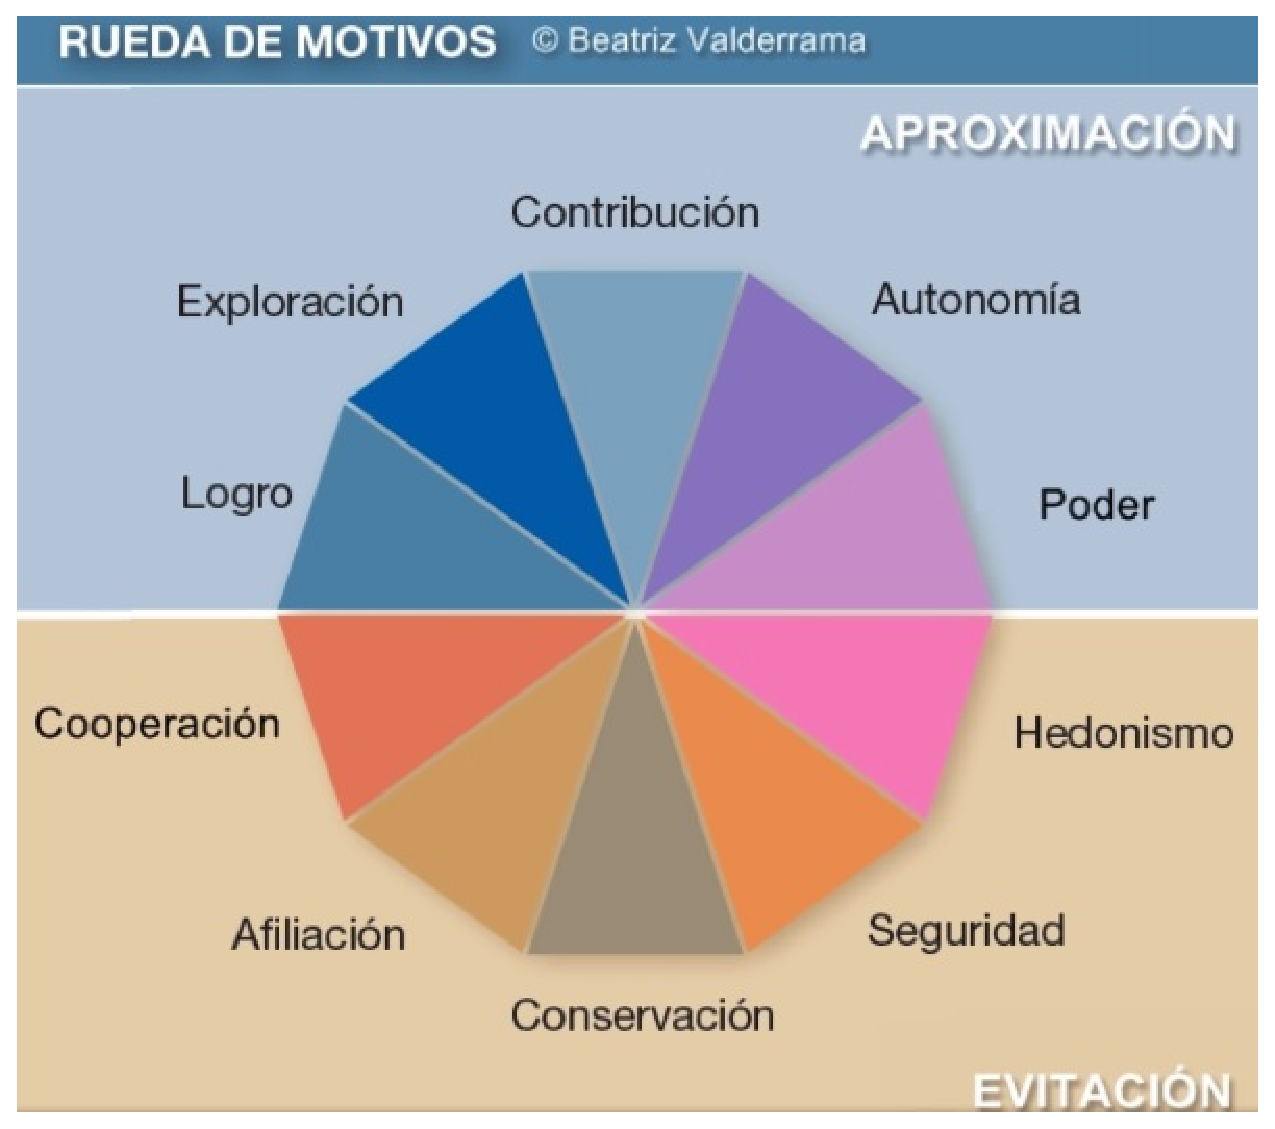
\includegraphics[width=0.5\textwidth]{02Antecedentes/contribucionesR/imagenes/rueda-de-motivos}
\end{figure}

Es así como tenemos en contra partes diferentes motivos dependiendo del jugador obejtivo, que son la búsqueda de:
\begin{itemize}
	\item Logros o hedonismo
	\item Exploración o seguridad
	\item Contribución o conservación
	\item Autonomía o afiliación
	\item Poder o cooperación
\end{itemize}
 
 
 

\subsection{Modelo de negocios en un videojuego}\label{modeloNegocio}
Para sustentar un proyecto o producto económicamente se debe tener claro un modelo de negocios. En el mundo de los videojuegos no existe la excepción, pero también debe considerarse que existen formas muy diferentes de adquirir el ingreso.

Incluso el mismo juego puede estar involucrado en un ingreso directo del servicio.

\subsubsection{Mercado global}
Se reporta segun Newzoo que 2.3 billones de jugadores en todo el mundo gastarán \$ 137.9 billones en juegos en 2018. Esto representa un aumento de + 13.3\% en comparación con el año anterior, o \$ 16.2 billones. Los ingresos por juegos digitales tomarán el 91\% del mercado global con \$ 125.3 mil millones, como podemos ver en la \cite{fig:merglo}
\begin{figure}
	\centering
	\caption{Mércado global al primer trimestre del año 2018}
	\label{fig:merglo}
	\includegraphics[width=0.5\textwidth]{02Antecedentes/contribucionesR/imagenes/merglo}
\end{figure}

Por primera vez, más de la mitad de todos los ingresos del juego provendrán del segmento móvil como vemos en la imagen{asdasd}. Los teléfonos inteligentes representarán el 80\% de esto, o \$ 56.4 mil millones, con el 20\% restante proveniente de tabletas.


\subsubsection{Presentación al cliente}
Un videojuego como cualquier software al momento de ser vendido al cliente puede encontrarse en dos presentaciones, una versión física o solo digital. En la siguiente tabla \cite{fiDi} se muestran las diferencias más destacables.

\begin{table}[htbp]
	\centering
	\caption{Tabla comparativa de un producto físico o digital}
	\label{fiDi}
	\begin{tabular}{lll}
		& Físico          & Digital     \\
		Coste de desarrollo                                   & sí              & sí          \\
		Coste de producción                                   & sí              & no          \\
		Coste de envío                                        & sí              & no          \\
		Riesgo de sobra/infra producir inventario             & sí              & no          \\
		Facturación por unidad vendida                        & mucho mayor     & mucho menor \\
		Unidad vendida costea soporte                         & generalmente sí & imposible   \\
		Porcentaje del precio de venta que percibe la empresa & 30\%-40\%       & 70\%        \\
		Tiempo de cobro                                       & 90 días o más   & 30 días     \\
		Capacidad de llegar al público con marketing          & caro            & difícil
	\end{tabular}
\end{table}

Aún así cabe mencionar que este es un aspecto general que involucra a cualquier software.

\subsubsection{Formas de ingreso}
Dentro de los videojuegos existen modelos de negocio que han dio cambiando a lo largo de los años y muchas de las veces depende del tipo del juego. Pero podemos definir las siguientes conforme lo visto y consumido en los últimos 5 años a la fecha del proyecto a presentar.

\begin{table}[htbp]
	\centering
	\caption{Tabla comparativa de ventajas y desventajas de modelos de negocios de videojuegos}
	\label{tablaMoneVJ}
	\begin{tabular}{llll}
		Nombre       & Descripción                                                                                                               & Ventaja                                                                                                                                                                                                                                                                                                                  & Desventaja                                                                                                                                                                                                                                                                                                                                                                            \\
		Pay-to-play  & Se debe pagar contenido y uso del videojuego                                                                              & \begin{tabular}[c]{@{}l@{}}* Rápido retorno de inversión\\ \\ * Sin limitación de juego\\ \\ * Puede re-dirigirse a otro modelo en caso de fracaso \\ \\ * Puede ser un producto físico, por lo que puede cobrarse contenido extra\\ \\ * Complementa con compras in-game\end{tabular}                                   & \begin{tabular}[c]{@{}l@{}}* No compras por desconocimiento del juego (más en móviles)\\ \\ * Inversión grande por enfoque a consolas \\ \\ * Jugadores esperan contenido de entretenimiento de larga duración y calidad\\ \\ * No hay soporte o cambios en el juego\\ \\ * Si es un producto físico debe costearse la producción\\ \\ * Necesita publicidad\end{tabular}             \\
		Free-to-play & Ofrece gratis contenido y uso del videojuego en su totalidad, se monetiza con publicidad y compras in-game                & \begin{tabular}[c]{@{}l@{}}* Contacto con los jugadores más rápido\\ \\ * Preferente para móviles\\ \\ * Preferente para juegos de poca inversión (que quiera escalar)\\ \\ * Complementa con compras in-game\end{tabular}                                                                                               & \begin{tabular}[c]{@{}l@{}}* Depende de la cantidad de jugadores activos\\ \\ * Debe ser un juego con adicción para sustentarse\\ \\ * Debe ser un juego “infinito”\\ \\ * Requiere continuas actualizaciones si desea mantenerse\\ \\ * Debe darse al jugador contenido nuevo a jugar\end{tabular}                                                                                   \\
		Freemium     & Ofrece gratis el uso del videojuego pero no se accede a todo su contenido, establece jerarquización de tipos de jugadores & \begin{tabular}[c]{@{}l@{}}* Conveniente para demos (versión lite)\\ \\ * Oportunidad de dar a conocer el juego\\ \\ * Oportunidad de convencimiento al jugador\\ \\ * Contacto con los jugadores más rápido\\ \\ * Preferente para móviles\\ \\ * Viable aun sí existen pocos jugadores dispuestos a pagar\end{tabular} & \begin{tabular}[c]{@{}l@{}}* Debe crearse contenido de calidad por pago\\ \\ * Debe existir un control y registro de jugadores para su jerarquización\\ \\ * Usualmente el contenido extra debe ser descargado de internet (por lo que implicaría otros gastos y recursos)\\ \\ * Recomendable ser un juego “infinito”\\ \\ * A veces requiere continuas actualizaciones\end{tabular} \\
		Suscripción  & Se debe pagar el contenido y uso del videojuego pero con limitaciones.                                                    & \begin{tabular}[c]{@{}l@{}}* Es combinable con otros modelos como el freemium\\ \\ * Permite a los jugadores explorar el juego completo por cierto tiempo\\ \\ * Oportunidad de dar a conocer el juego\end{tabular}                                                                                                      & \begin{tabular}[c]{@{}l@{}}* Debe crearse contenido de calidad por pago\\ \\ * Recomendable ser un juego “infinito”\\ \\ * A veces requiere continuas actualizaciones\\ \\ * Debe darse al jugador contenido nuevo a jugar\\ \\ * Depende de la cantidad de jugadores activos\\ \\ * Debe ser un juego con adicción para sustentarse\end{tabular}                                    
	\end{tabular}
\end{table}

\subsubsection{Ingredientes de monetización}
Los modelos de negocio anteriores pueden ser combinables con otros "ingredientes" de monetización para acrecentarlos ingresos. 
\begin{itemize}
	\item Dinero virtual: Es el medio de intercambio que utiliza un videojuego para poder formalizar las compras dentro de él. A menudo se suele diferenciar el virtual currency (dinero virtual que se consigue por las propias mecánicas del juego y con abundancia) y el hard currency (dinero virtual premium que se consigue con dinero real o con acciones muy concretas y con mucha escasez).
	\item Bienes virtuales: Son objetos intangibles que son comprados e intercambiados que sólo tienen sentido dentro del juego, muchas veces estos son comprados con dinero virtual. 
	\item Publicidad y patrocinio: Anuncios o productos presentados en el juego para darse a conocer.
	\item Bonificaciones y servicios virtuales: Son aceleradores de juego o servicios que mejoran el desempeño o facilitan en el juego.
	\item DLC (downloadable content): Es un contenido de descarga digital exclusivo y adicional de un videojuego que se vende por separado y posterior al lanzamiento de este. Suele lanzarse para alargar la longevidad del videojuego y para aprovechar su éxito comercial. Su adquisición no tiene sentido sin tener antes el videojuego ya que es un producto complementario y dependiente a él.
\end{itemize}

\section{Costo de hacer un videojuego}\label{costoVJ}

	
\subsubsection{Salarios}
Pararealizar un videojuego se necesita de diferentes profesiones parallevarlo a cabo.
En el siguiente cuadro se mostrará la profesion y salario a recibir en la industria del videojuego en una empresa ya establecida al año 2014 segun la encuesta ____ con una relación definida en experiencia.


\begin{table}[]
	\centering
	\caption{My caption}
	\label{my-label}
	\begin{tabular}{lllll}
		Rama                                                      & Profesión                   & Salario con \textless 3años de exp. & Salario con 3-6años de exp. & Salario con \textgreater 6años de exp. \\
		\multirow{3}{*}{Programadores e ingenieros}               & Programador                 & \$71,855 USD                        & \$79,877 USD                & \$103,789 USD                          \\
		& Programador principal       &                                     & \$94,877 USD                & \$116,151 USD                          \\
		& Director técnico            &                                     &                             & \$135,781 USD                          \\
		\multirow{3}{*}{Artistas y animadores}                    & Animador                    & \$50,000 USD                        & \$55,547USD                 & \$82,230 USD                           \\
		& Artista principal           &                                     & \$71,029 USD                & \$71,87576 USD                         \\
		& Director de arte            &                                     &                             & \$110,000 USD                          \\
		\multicolumn{1}{c}{\multirow{2}{*}{Diseñadores de juego}} & Diseñador de juego          & \$53,000 USD                        & \$65,516 USD                & \$77,768 USD                           \\
		\multicolumn{1}{c}{}                                      & Director creativo           &                                     & \$68,654 USD                & \$101,944 USD                          \\
		\multicolumn{1}{c}{\multirow{3}{*}{Productores}}          & Productor asociado          &                                     & \$59,079 USD                & \$61,912 USD                           \\
		\multicolumn{1}{c}{}                                      & Lider de proyecto           &                                     & \$73,500 USD                & \$93,160 USD                           \\
		\multicolumn{1}{c}{}                                      & Productor ejecutivo         &                                     &                             & \$126,833 USD                          \\
		Profesional de audio                                      & Director de sonido          &                                     &                             & \$109,500 USD                          \\
		\multicolumn{1}{c}{\multirow{2}{*}{Testers}}              & Tester                      &                                     & \$38,833 USD                &                                        \\
		\multicolumn{1}{c}{}                                      & Lider de control de calidad &                                     & \$60,417 USD                & \$65,500 USD                           \\
		\multirow{3}{*}{Negocios y administración}                & Marketing                   &                                     & \$73,500 USD                &                                        \\
		& CEO                         &                                     &                             & \$135,735 USD                          \\
		& Gerente ejecutivo           &                                     &                             & \$156,731 USD                         
	\end{tabular}
\end{table}


\subsection{Modelo de datos}
La primera observación en atender fue el modelo de datos del juego, dicho modelo
de datos se realizó utilizando un modelo entidad relación de base de datos (Ver
Anexo \ref{Anexo:ModeloDatos}) ya que al modelarse de esta forma hace escalable
el juego si se deseara en algún futuro emplear una base de datos para mejorar
el almacenamiento de datos y el manejo de más usuarios para ofrecer un modo
online. El modelo de datos está basado en el modelo de clases y contiene
únicamente a las clases actoras. Toda entidad actora se define como una
especialización de una entidad base llamada GameObject, esta entidad está
definida por como su identificador y por otras entidades como GameObjectPosition,
Level, Tag, AnimationMachine, entre otros.

\subsection{Estrategias para combatir la adicción entre los usuarios}
La segunda observación sobre la que se trabajo fue como disminuir la adicción
del jugador al videojuego Yolotl. Esta observación dio lugar a una investigación
sobre la adicción a los videojuegos ya que antes de proponer alguna solución se
debía conocer cómo se definía, las causas y las consecuencias de la adicción al
videojuego. Al final de la investigación se pudieron formular tres posibles
soluciones para evitar la adicción del jugador; sin embargo, dado que este tópico
no estaba en la planeación original del proyecto y por el trabajo que
conlleva cada una de las soluciones se decidió únicamente describir las
soluciones y sus implicaciones sin desarrollar ninguna de las tres. A continuación,
se describen a manera de resumen las soluciones (nuevamente si se dese a
profundizar en la investigación realizada y las soluciones se puede consultar
el Anexo \ref{Anexo:AdiccJuga}):
    \begin{itemize}
        \item \textbf{Notificación de confirmación para continuar la partida.} Esta
        solución propone que el juego solicite la confirmación del usuario para
        continuar una vez que éste ha detectado que el jugador ha estado jugando
        durante un tiempo prolongado como una hora.
        \item \textbf{Control paterno.} El juego le envía un formulario al tutor del
        jugador por medio de un correo electrónico. En este formulario el tutor podrá
        decidir cuánto tiempo al día la aplicación podrá estar abierta.
        \item \textbf{Sistema de vidas.} El jugador tiene una cantidad de vidas
        limitadas. Cada vez que el jugador ingresa a un nivel o muere dentro de
        uno y reinicia la partida se gasta una vida. Para recuperar vidas el
        jugador deberá de esperar un determinado tiempo.
    \end{itemize}



\section{Trabajo realizado durante trabajo terminal 1} \label{TrabajoTerminal1}
En esta sección se habla a manera de resumen el trabajo realizado durante el 
periodo correspondiente a trabajo terminal 1. La división de esta sección 
queda organizada en dos subsecciónes: una para la etapa de preprodución y 
otra para los dos primeros \textit{sprints} de la estapa de produción. 

\subsection{Etapa de Preproducción}\label{EtapaPreproduccion}
Esta etapa corresponde a la planeación analisis y diseño del juego. Como lo indica 
la metodología \textit{Huddle}, para esta etapa se trabaja en el desarrollo del 
documento de diseño del juego. Esta etapa queda del desarrollo queda dividida en 
cuatro \textit{sprints}.

\subsubsection{Primer Sprint Huddle de Preproducción}\label{Prepro01}
Antes de iniciar el diseño del juego se realiza un trabajo de investigación 
sobre la cultura azteca. Esta investigación abarca:
\begin{itemize}
        \item \textbf{La sociedad mexica:} su historia tradiciones y clases sociales. 
        \item \textbf{Mitología mexica:} Dioses, mito de los cinco soles, mito de la 
        creación del hombre del maíz, el Mictlán.
        \item \textbf{Historia de la Malinche:} Historia del personaje antes y después 
        de la llegada de los españoles.
\end{itemize} 
 
Durante la etapa de investigación se selecciona la información histórica que 
sera relevante y útil para la narrativa del juego y el diseño de su jugabilidad. 
Para la investigación histórica de esta etapa se consultan libros, códices, 
páginas de Internet, artículos de investigación e incluso se visitan museos 
como el templo mayor.

\subsubsection{Segundo Sprint Huddle de Preproducción}\label{PrePro02}
En este \textit{sprint} se redactan las primeras secciones del documento de diseño del 
juego \textit{Yolotl}. Se inicia con la idea concepto y con el tema del juego. De igual 
forma se selecciona un nombre para el juego a desarrollar: \textit{Yolotl}. 
Para algunos juegos la mecánica es la primera es ser definida; no obstante, 
por la naturaleza del juego como herramienta de transmisión de cultura, 
\textit{Yolotl} nace con su historia. La historia de \textit{Yolotl} pasa por 
diferentes etapas de diseño; siendo modificada gradualmente, pero manteniendo 
algunos elementos clave como la lucha contra la divinidad. 
\\
\par
En la etapa del concepto también se define la plataforma para la que será 
el juego: dispositivos móviles con sistema operativo Android 5.2. Por su parte 
se decide utilizar un motor de juego como herramienta de desarrollo, pues esto 
permite centrarse en el diseño e implementación de aquellos elementos que 
diferencien a \textit{Yolotl} del resto de juegos, tal como su mecánica, sus 
personajes, etc. Luego de investigar sobre los motores de juegos disponibles, 
se elije Unity 3D como ambiente de desarrollo.
\\
\par
Una vez teniendo la idea concepto se define la visión del juego y sus mecánicas. 
En cuestión de las mecánicas el enfoque por el que se opta es el de mantener 
el juego con mecánicas simples y familiares para aquellos jugadores que ya habían 
tenido alguna experiencia con algún juego de plataformas, sin descartar algunos 
detalles que le dieran identidad al juego en cuanto a su jugabilidad. Paralelamente 
a la preproducción, se inicia el desarrollo de un primer demo con el fin de 
familiarizarse con la herramienta de Unity3D, este demo incluye las mecánicas más 
simples del juego.
\\
\par
Con la historia, la visión y la mecánica definidas se procede a puntualizar los 
estados del juego, diseñar las interfaces gráficas de navegación y de interacción 
con el personaje. Para ver la versión final de las interfaces se puede consultar 
anexo \ref{Anexo:Intefaces}.

\subsubsection{Tercer Sprint Huddle de Preproducción}
En el tercer Sprint se definen la cantidad de niveles y en que consiste
cada uno, de igual forma se establecen los objetivos de cada nivel, la recompensa 
a obtener una vez completado el mismo, los enemigos a vencer y las cinemáticas que 
fungen como transiciones entre niveles.  
\\
\par
Al mismo tiempo que se diseñan los niveles, se detallan los 
personajes tanto a nivel narrativo como a nivel de jugabilidad, definiendo habilidades 
para los enemigos, los niveles en los que parecerían y sus acciones dentro de 
la historia. Para esta parte se trata de obtener la mayor fidelidad posible a 
los mitos y códices. En el anexo \ref{Anexo:Personajes} se habla a mayor detalle 
sobre el diseño de los personajes.

\subsubsection{Cuarto Sprint Huddle de Preproducción} 
En el cuarto sprint se termina de escribir el argumento del juego, de esta 
destapa se obtiene el guión literario del juego. En este \textit{sprint} también se definen 
elementos de ambientación para el juego tales como la música de fondo, los 
efectos de sonido y los efectos especiales. 
\\
\par
De igual forma, en este \textit{sprint} se especifican las armas de los personajes, los 
ítems; quedando diseñados tanto a nivel de comportamiento como a nivel 
visual. Al igual que con los personajes se busca que las armas, tanto en 
comportamiento como en diseño, se mantengan lo más fiel posible a los mitos 
y leyendas de donde se basaron.
\\
\par
Con el cuarto \textit{sprint} se finaliza la etapa de preproducción, obteniendo así un 
documento de diseño lo suficientemente detallado como para iniciar el diseño 
del juego a nivel de ingeniera. 

\subsection{Etapa de producción}
En esta sección se habla del trabajo realizado durante los dos primeros 
\textit{sprints} de esta etapa, ya que fueron desarrollados durante los meses 
correspondientes al trabajo terminal 1. Todos los \textit{sprints} del la etapa 
de producción posteriores al segundo \textit{sprint} son abordados en la sección 
\ref{TrabajoTT2}.

\subsubsection{Primer Sprint Huddle de Producción.}
En este \textit{sprint} se realiza un análisis del documento de diseño, en consecuencia 
de este análisis se se diseña el videojuego en materia de las clases que lo 
componen y el modelo bajo el que funcionaría el juego a nivel de programación. 
\\
\par
Haciendo uso del paradigma orientado a objetos se propone emplear tres tipos 
de clases:
\begin{itemize}
        \item \textbf{Actores:} Son las clases que modelan a los enemigos, los ítems, 
        los coleccionables, los checkpoints y al jugador.
        \item \textbf{Controladores:} Son las clases encargadas de gestionar la partida 
        y la navegación entre interfaces. Estas clases desencadenan eventos conforme a 
        las acciones de las clases actoras. Estas clases también son las encargadas de 
        verificar que se cumplan las reglas de los niveles.
        \item \textbf{Auxiliares:} Estas clases ayudan al funcionamiento de los actores 
        y los controladores. Estas clases también se encargan le vincular datos con 
        las clases controladoras como efectos de sonido, música, datos para la 
        progresión entre niveles.
\end{itemize}
El modelo planteado permite reutilizar parte del demo generado durante la etapa 
de preproducción. Por lo aque en este \textit{sprint} se inicia la integración 
del código del primer demo con el comportamiento modelado por las clases definidas 
en el párrafo anterior. 
\\
\par
En el primer \textit{sprint} de Producción también se crean los \textit{sprites} del 
primer nivel utilizando la herramienta de modelado en \textit{3D Blender}. Al 
finalizar este \textit{sprint} se determina la no viabilidad del modelado en 3D de los 
\textit{sprites} por cuestiones de tiempos; en consecuencia, se descarta este 
método para generar los \textit{sprites} y se inicia el desarrollo de los 
\textit{sprites} a partir de otras técnicas de animación más tradicionales.

\subsubsection{Segundo Sprint Huddle de Producción.}
En este \textit{sprint} se inicia el desarrollo de los \textit{sprites} con \textit{Adobe Photoshop} 
y \textit{Corel Draw}. A la par se inicia la maquetación de la etapa de selva 
del nivel uno. En este sprint se logran terminar todos los \textit{sprites} referentes 
al primer nivel del juego tales como: 
\begin{itemize}
        \item Objetos de fondo: Arbustos, árboles, jarrones y cajas. 
        \item Imagen de fondo: Fondo de la selva, la ciudad y el menú principal. 
        \item Ciudadanos del mercado: Comerciantes, nobles y esclavos. 
        \item \textit{Xólotl} en su forma \textit{xoloitzcuintle}: Bloques de 
        animacion para correr y normal.
        \item \textit{Malinalli} sin la caracola: Bloques de animación correr, 
        saltar y normal.
\end{itemize}
Una vez terminados los \textit{sprites} referentes al nivel uno estos se integran al código 
permitiendo tener un segundo prototipo con la siguiente funcionalidad:
\begin{itemize}
        \item Control de personaje por medio de la GUI.
        \item Transiciones entre interfaces.
        \item Personaje seguible que aparece en el primer nivel funcional.
        \item Funcionamiento básico del controlador de diálogos.
\end{itemize}

